\section{Power Quality Monitoring}
Electric power is often seen as self-evident. It can be consumed at any time and any point all over the country. But, this standard of comfort implies a lot of effort for the power suppliers. The wide variety of power producers makes it hard for the suppliers to deliver a power grid with stable frequency and voltage. On the one hand, nuclear power plants produce a stable high amount of baseline power, on the other hand highly dynamic techniques like solar or wind energy can make the grid unstable.
As a result, the grid has to be balanced. Surplus power has to be compensated, for example by pumping water into big artificial lakes in the mountains. Especially the increasing use of electric equipment in private and industrial environments punctuates the need for a stable power grid.

To fulfill the task of keeping the grid stable, precise measurement is needed at defined points in the power grid. Therefore, the term power quality monitoring describes the the monitoring of important parameters of the power grid, such as frequency or different aspects of the voltage. Furthermore, analysis are made to react to imbalances and to predict further events like the outage of a component of the power grid.


The European Standard EN 50160 defines the parameters of the power supply network that have to be monitored to ensure the given limits by the standard. The standard describes the characteristics under normal operation conditions at a supply terminal from a customer to the public network. The following sections describes some example characteristics of the corresponding Austrian standard \"OVE/\"ONORM EN 50160\cite{en50160}. Furthermore, the International Standard IEC 61000-4-30 defines testing and measurement techniques for power quality monitoring. \cite{iec61000}


The goal of the proposed thesis is to develop a measurement system that measures relevant characteristics of a power system for power network supplier. According to the underlying standard (EN 50160), it is sufficient to capture the voltage on a power line to calculate the relevant properties for a power quality analysis. The scenario used in the thesis consist of synchronized measurement devices, distributed over a wider geographical area, that are connected to a cloud system. The cloud system provides functionality for managing the devices and visualization of the measured data. Furthermore, interfaces can be consumed to use the data with external systems. With this design, the power quality of a power supplier network can be captured.

\subsection{Parameters}
\subsubsection{Effective Value}
The effective value of the power supply voltage has to be 230 V $\pm$ 10\% in 95\% of every 10 ten minute interval and 230 V + 10\%/- 15\% in every ten minute interval.
The following formula is used to calculate the effective value of the captured signal:

\[ U_{eff} \approx \sqrt{\frac{1}{n} \sum_{n=0}^n x_i^2 } = \sqrt{\frac{1}{n} (x_1^2 + x_2^2 + x_3^2 + \dots + x_n^2)} \]
\newline
In order to calculate the following characteristics, a Fourier transformation (see \ref{fft} for further information) has to be applied to the captured data.

\subsubsection{Frequency}
The frequency of the power supply voltage has to be 50 Hz $\pm$ 1\% at 99.5\% of the year and 50 Hz + 1\%/- 6\% at 100\% of the year. After the Fourier transformation, the frequency with the highest amplitude is assumed to be the fundamental frequency $f_0$.

\subsubsection{Voltage harmonics}
According to the standard, all voltage harmonics up to the $25^{th}$ order has to be monitored. Each value has to be calculated over an interval of ten minutes and has to be tested against the values listed in the standard as described in appendix \ref{app:en50160}. After the fundamental frequency $f_0$ is extracted out of the results of the Fourier transformation, the voltage harmonics can be calculated. The frequencies of the corresponding harmonics can be calculated by $f_n = n \cdot f_0$. The voltage harmonics of the desired order can then be calculated by the following formula:

\[ V_n = \frac{A(f_n)}{A(f_0)} \cdot 100\% \]
\newline
where $A(f_n$) is the amplitude of the signal at the frequency $f_n$.

\subsubsection{Total harmonic distortion}
In addition to the voltage harmonics, the total harmonic distortion (THD) has to be $\leq$ 8\%. For this, the voltage harmonics up to the $40^{th}$ order are aggregated by using the following formula: 

\[ {THD} = \frac{\sqrt{\sum_{h=2}^{40} V_h^2}}{V_1} \cdot 100\% = \frac{\sqrt{V_2^2 + V_3^2 + V_4^2 + \dots + V_{40}^2}}{V_1} \cdot 100\% \]

\subsection{Measuring Electric Characteristics}
\todo{better title}

To calculate the selected power quality characteristics, the voltage of the power line has to be monitored. In order to accomplish this task, the analog signal has to be digitized for further computational processing. The signal has to be sampled and each sample has to be quantized to a finite number of bits representing the sample in a digital way. The accuracy of the quantization process strongly depends on the number of bits that such an analog/digital converter (ADC) offers. Assume an ADC represents a sample by $B$ bits, the sample is transformed to a value in the range of $2^B$ bits, furthermore, the full-scale range $R$ has to be taken into account. As a result of this, the full-scale range $R$ is divided in $2^B$ steps and the resulting quantization with or quantization resolution can be represented using the following formula\cite{sig_proc}:
\[ Q = \frac{R}{2^B} \]
\newline
In the proposed scenario, a ADC with a $R$ = $\pm$ 1200 V = 2400 V and $B$ = 24 bits is used. This results in the following quantization resolution:
\[ Q = \frac{2400 \; V}{2^{24} \; bits} = 0.000143 \; V \approx 143 \; \mu V \]
\newline
Beside having a efficient quantization resolution, choosing the right sample rate is crucial. In order to reconstruct the measured signal, the time between two sample has to be chosen in a manner that on the one hand, unnecessary often taken samples of the same signal level are generated (oversampling) and on the other hand, not too less samples are taken such that the original signal cannot be reconstructed (undersampling)\cite{sig_proc}. To avoid undersampling, the Nyquist sampling theorem has to be applied: Taken a real signal, that is bandlimited to $B$ Hz (only signals with a frequency below $B$ Hz are sampled), can be reconstructed without errors with the frequency $R$, described by the following formula\cite{sampling}:
\[R > 2 \cdot B\]
\newline
In the proposed scenario, we examine total harmonic distortion up to the $40^{th}$ order or harmonics. According to the standard, the maximal allowed frequency is 50 Hz + 1\% = 50.5 Hz. Therefore, the $40^{th}$ harmonic has a frequency of at most 2020 Hz. The signal is bandlimited by a lowpass filter to $B$ = 5000 Hz. According to the Nyquist sampling theorem, the sample frequency has to be set to at least $R > 2 \cdot B = 10000$ Hz. Hence, the sample frequency of the measurement device used to evaluate the scenario is set to 20000 Hz.

\subsection{Transformation from Time- to Frequency Domain}

\label{fft}
Since a great number of important characteristics of the power quality depends on measuring the frequency (and it's components) on a power line, the transformation form a signal recorded in the time domain to it's frequency parts shall be discussed.
The most important method used for transformation is the Fourier transform. By using the Fourier analysis, a signal can be represented by its sinusoidal waveforms. In other words, the output of the Fourier analysis shows the amplitude and phase (cosine and sine components) at every frequency of the original signal. The conversation of a signal from the time- to the frequency-domain can be represented by the Discrete Fourier Transform (DFT). The input for the DFT is a signal of $N$ points and can be calculated using the following formula\cite{fourier}:
\[ X(k) = \frac{1}{N} \sum_{n=0}^{N-1} x(n) e^{-j \frac{2 \pi}{N} nk} \]


Implementing the DFT directly results in an algorithm with a complexity of $\mathcal O(N^2)$. Therefore, efficient implementations (Fast Fourier Transform - FFT) are available that reduce the complexity to $\mathcal O(N \cdot log(N))$. The most common FFT algorithm is the Cooley-Tukey algorithm that uses the divide and conquer approach which can be found in listing \ref{cooley_tukey_impl}\cite{cooley_tukey}. The results of this transformation are 'Bins' representing a sample of the spectrum with the frequency

\[f_i = \frac{R}{N} \cdot i \]
where $i$ is the current Bin-index. Therefore, the output of the FFT has a limited resolution of the frequency. In the proposed scenario, the resolution (or the difference between two Bins) should be at least 0.5 Hz which can be represented as $\Delta f = f_{n} - f_{n-1} = $ 0.5 Hz. Since $n \geq 0 $ and $n < N$, we can choose an arbitrary $n$ in this range.

\[ n = 2, R = 20000 Hz \]
\[ \Delta f = f_{n} - f_{n-1} = f_{2} - f_{1} \]
\[ \Delta f = \frac{R}{N} \cdot 2 - \frac{R}{N} \cdot 1 = \frac{2 \cdot R - 1 \cdot R}{N} = \frac{R}{N} \]
\[ \Rightarrow N = \frac{R}{\Delta f} = \frac{20000 Hz}{0.5 Hz} = 40000 \]

When looking at the recursive algorithm, it can be seen that the algorithm works efficiently when $N$ is a power of two. Hence we take the next greater power of two for $N$. $N = 2^{16} = 65536$, which results in a resolution $\Delta f = $ 0.305 Hz.
\newline
\newline
For the sake of completeness, 'Window functions' have to be taken into account. The FFT works under the precondition that the signal is periodic in the examined window ($N$ points). Due to measurement uncertainty and that in practice, the signal is not a perfect sine wave, errors occur in the output. To minimize the error, window function can be applied to the measurement data before FFT, which transforms the input signal to a periodic signal. Different window function (Hanning, Hamming, Blackman, etc.) exists to examine different aspects of the spectrum. Practice has shown that the Hanning-Window is useful in most situations and is also applied in the proposed thesis. Every sample $x[n]$ in the time domain is multiplied with $w[n]$, which has the following formula\cite{signalverarbeitung}:

\[w[n] = 0.5 - 0.5 \cdot cos(\frac{2 \pi n}{N})\]

A common implementation of the FFT algorithm is the recursive version of Cooley and Tukey. The complex signal input array is splitted in two arrays. One with the even indices, one with the odd indices. After that, the function is called again on this two arrays until the length of the input array is less or equal 1. After the recursion returns, the calculation of the frequency-domain data is made by appliying .... \todo{cite}

\lstset{language=C++, caption={Recursive Cooley-Tukey FFT algorithm}, label={cooley_tukey_impl}, numberstyle=\footnotesize,
								basicstyle=\ttfamily,
                keywordstyle=\color{blue}\ttfamily,
                stringstyle=\color{red}\ttfamily,
                commentstyle=\color{green}\ttfamily,
                morecomment=[l][\color{magenta}]{\#}}
\begin{lstlisting}[frame=single]
private void CalculateFFT(ref Complex[] signal)
{
	int n = signal.Length;

	if (n <= 1)
	{
		return;
	}

	//Divide
	Complex[] even = new Complex[n / 2];
	Complex[] odd = new Complex[n / 2];

	for (int i = 0; i < n / 2; i++)
	{
		even[i] = signal[2 * i];
		odd[i] = signal[2 * i + 1];
	}

	//Conquer
	CalculateFFT(ref even);
	CalculateFFT(ref odd);

	//Combine
	for (int i = 0; i < n / 2; i++)
	{
		double kth = -2 * i * Math.PI / n;
		Complex wk = new Complex(Math.Cos(kth), Math.Sin(kth));

		signal[i] = even[i] + wk * odd[i];
		signal[i + n / 2] = even[i] - wk * odd[i];
	}
}
\end{lstlisting}
\todo{cite}
\section{Cloud Computing}

\epigraph{''I don’t need a hard disk in my computer if I can get to the server faster\dots \\ carrying around these non-connected computers is byzantine by comparison.''}{--- \textup{Steve Jobs}, former Apple CEO}

\subsection{Cloud Characteristics}
The essential characteristics of cloud computing are as follows\cite{cloud_characteristics}\cite{nist}:

\subsubsection{On-demand self-service}
Allows users of the cloud to consume capabilities from it. Common capabilities are network storage, server time or applications. The big difference compared to other computing models is, that the capabilities can be consumed as needed without complex interaction with the cloud provider. 

\subsubsection{Broad network access}
All of the capabilities can be accessed over the network by standard mechanisms. Furthermore, thin and thick client platforms are supported (from mobile devices up to workstations).

\subsubsection{Resource pooling}
The cloud provider's resources are pooled together to serve multiple consumers. End users of the cloud mostly need not to know the location of the data center hosting the cloud environment (often users can choose the country or a certain datacenter). The different physical and virtual resources are assigned and reassigned dynamically on demand.

\subsubsection{Rapid elasticity}
For rapid elasticity and scalability, the provisioned capability can be automatically scaled up and down. For the end users, capabilities are often presented as unlimited.

\subsubsection{Measured service}
For billing purposes and transparency for both the cloud provider ant the end user, measuring capabilities are applied. Furthermore, automatic control and optimization of the resources are performed based on this measures.

\subsection{Service Models}
By definition, the cloud system can be divided into the following three service models\cite{nist}:

\subsubsection{Software as a Service (SaaS)}
Software is provided to the users within the cloud infrastructure. To use the software, the services provided by the cloud can be accessed by either a web interface or is integrated into software installed locally. The advantage of this service model is, that the users consuming the services of the cloud rely on the underlying hardware (physical servers or network interfaces) and software (operating systems or databases)\cite{nist}.
		
Examples: Google Mail, Google Docs\cite{trustedcloudcomputing}.

\subsubsection{Platform as a Service (PaaS)}
Software created by users can be deployed to the cloud. For this, the cloud provides libraries, services and tools to support the users by developing a software with a programming language supported by the cloud. Like before, the underlying hard- and software is maintained by the cloud operator\cite{nist}.
	
Examples: Google App Engine, Windows Azure\cite{trustedcloudcomputing}. 

\subsubsection{Infrastructure as a Service (IaaS)}
The users can consume computational power from the cloud. This includes the use of servers and operating systems, storage solutions, networking resources or additional capabilities like processing power. Again, the underlying hard- and software is maintained by the cloud operator\cite{nist}.
	
Examples: Amazon Elastic Compute Cloud (EC2), Amazon Simple Storage Service (S3)\cite{trustedcloudcomputing}.

Figure \ref{fig:cloud_stack} shows the three main service models and the responsible entities for the involved services.

\begin{figure}[h]
	\centering
		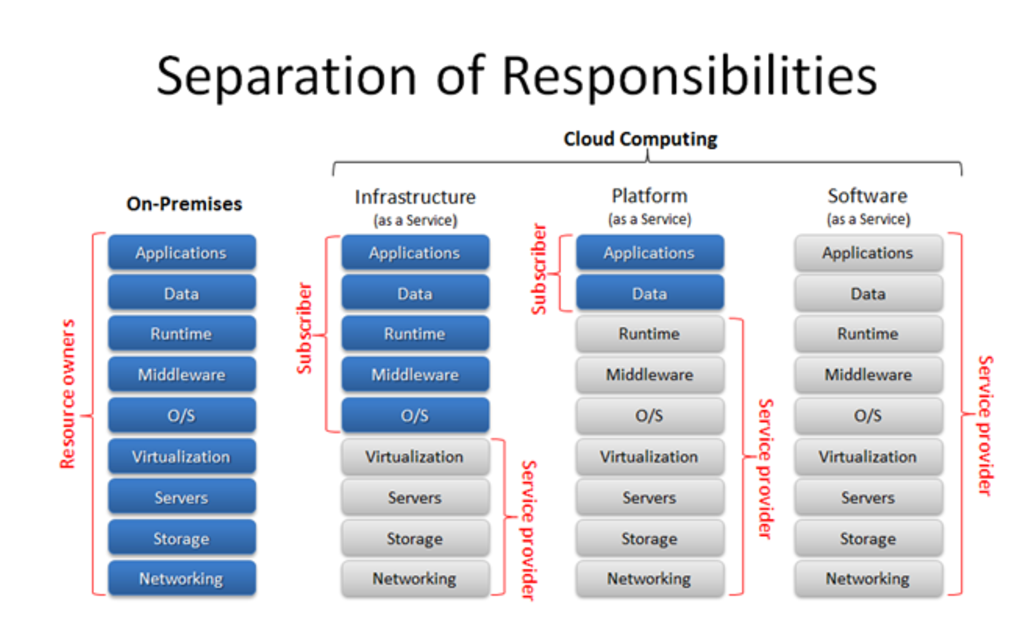
\includegraphics{graphics/service_models.eps}
	\caption{Service models\cite{trustedcloudcomputing}}
	\label{fig:cloud_stack}
\end{figure}

\todo{\url{https://blogs.technet.microsoft.com/yungchou/2010/11/15/cloud-computing-primer-for-it-pros/}}


Furthermore, the following subset of service models can be derived from the Everything as a Service (XaaS) aspect:

\subsubsection{Data Storage as a Service (DaaS)}
DaaS can be seen as enhancement of IaaS. The main idea behind this model is to provide storage solutions to users. Often supported services are databases (RDBMS or other types) and file storage.
		
Example: Amazon Simple Storage Service (S3)\cite{issues}.

\subsubsection{Human as a Service (HuaaS)}
Services, that rely on information generated by a crowd of people. Human intelligence is used to fulfill tasks that are provided as a service to the users. Persons in the crowd use their tools, skills or knowledge to solve a task or a small subset of a task. The cloud systems aggregates the single results and provide as a service to the users.
	
Example: Amazon Mechanical Turk\cite{huaas}.

\subsubsection{Other models}
Since there is no strict separation between the stated service models, there exist various combination and modifications of them. The following listing shows some additional classification \cite{cloud_characteristics}.
\begin{itemize}
	\item Database-as-a-Service
	\item Security-as-a-Service
	\item Communication-as-a-Service
	\item Management/Governance-as-a-Service
	\item Integration-as-a-Service
	\item Testing-as-a-Service
	\item Business Process-as-a-Service
\end{itemize}

\section{Internet of Things}

When looking at the past, a clear separation of digital and physical industries can be observerd. Since 1990, the Internet gave new opportunities to non-digital industries by creating new business models. Around 2005, the term ``Web 2.0'' came up as a summarization for Social Media, Open Source, Crowdsourcing, etc, allowing users to contribute to content in the Internet. With ``Web 3.0'' (around 2015), the concept of the ``Internet of Things (IoT)'' was introduced with new business models like ``Digitally Charged Products'' or ``Sensor as a Service'' \cite{iotfleisch}.

The Internet of Things introduces hybrid solutions that merge physical objects and digital services, with the vision to connect every object and location to the Internet. To fullfill this task, objects are equipped with computational intelligence (computers) that can be access over the Internet (or other objects) to read and write information from and to a physical object. The object itself is called a ``Thing'', hence the Name ``Internet of Things'' and is now a composition of both the physical and digital world \cite{iotfleisch}.

By adding computational intelligence to a physical object, the value of the ``Thing'' is increased in many ways. From an academic view, the value creation can be seen as five layers called the ``Value-creation Layers'' and will be explained in the next section \cite{iotfleisch}.

\url{https://www.alexandria.unisg.ch/236057/1/2090_EN_Bosch%20Lab%20White%20Paper%20GM%20im%20IOT%201_2.pdf}
\subsection{Value-creation Layers}

Figure \ref{fig:value_creation_layers} shows the five layers of value-creation within the Internet of Things. To get a better understanding of what the five layers are responsible for, a smart lightbulb is used as an example.

\begin{figure}[h]
	\centering
		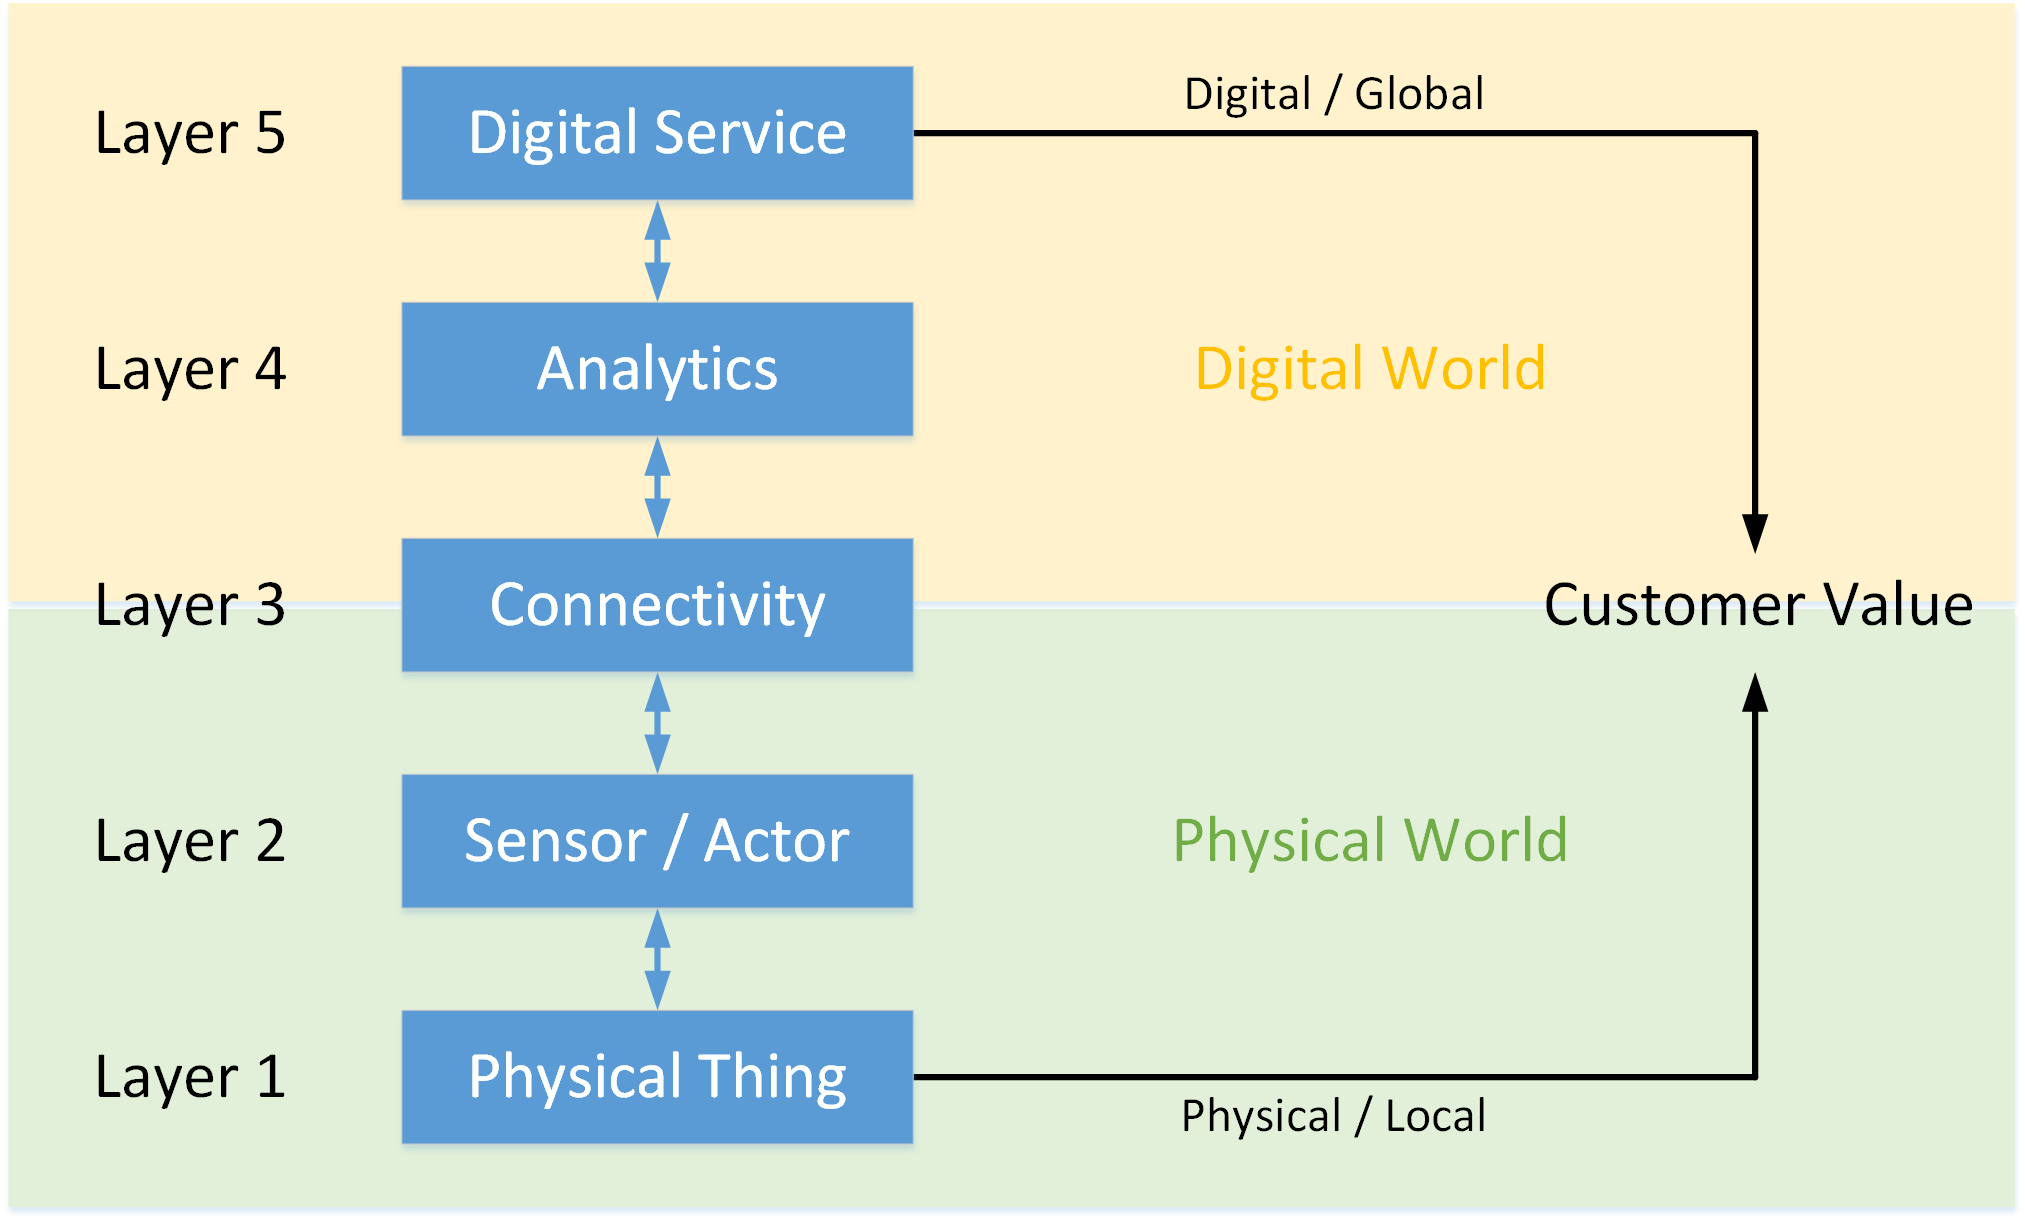
\includegraphics[scale=0.5]{graphics/iot_layers.eps}
	\caption{Value-creation Layers\cite{iotfleisch}}
	\label{fig:value_creation_layers}
\end{figure}

\subsubsection{Layer 1: Physical thing}
This layers describes the physical thing, e.g. a lightbulb. A thing is always bound to a location and has a direct benefit for the user (e.g. serving light). Since the location is fixed, it can only act in an immediate environment.

\subsubsection{Layer 2: Sensor/Actuator}
Layer 2 adds sensor and actuator elements to the thing. By adding a minicomputer to the physical object, the sensors can measure data and the actuators can deliver local services. In the proposed example, the sensor could measure the presense of a person and then switch of the lightbulb.

\subsubsection{Layer 3: Connectivity}
This layer connects the physical thing and the sensors/actuators to the Internet. Within this layer the device gets accessible via the Internet by, for example, a radio module that is connected to the local wireless network. By using modern technologies, this step can be done at marginal costs.

\subsubsection{Layer 4: Analytics}
In this layer, the collected data from the sensors are collected and stored for further processing (e.g. plausibility checks or classification). Additional web services can be integrated to generate actions for the actuators or add additional information to the sensor data. Usually this is achieved by using a cloud system. In this layer and additional value is added to the ``stupid'' thing. In the example this layer could derive motion patterns from the lightbulb.

\subsubsection{Layer 5: Digital service}
This layer combines all the previous layers and offers a functionality as a digital service. As an example, the lightbulb could be exposed to users all over the world via a wegbsite or a mobile application. On this layers new digital business model patterns can be applied.

By applying the previous layers to a physical object, the value of the thing is more than the sum of its parts. Connectivity to the Internet nowadays can be made at small costs. One important thing is, that the layers are not independent of each other. The flow of information has to pass the five layers always in both directions in order to ensure the additional value of the product.

\subsection{Business model patterns}

\subsection{Comparision with 'Industrial Internet of Things'}

\subsection{Comparision with 'Industry 4.0'}

\subsection{Impact on the thesis}
\todo{better title}